\documentclass[prd,twocolumn,superscriptaddress,nofootinbib,amsmath,amssymb]{revtex4-2}
% Physical Review D (network paper).  Build: latexmk -pdf main.tex  (needs revtex4-2 and apsrev4-2: texlive-publishers)
\usepackage[utf8]{inputenc}
\usepackage{graphicx}
\usepackage{booktabs}
\usepackage{xcolor}
\usepackage[colorlinks=true,linkcolor=blue!50!black,citecolor=blue!50!black,urlcolor=blue!50!black]{hyperref}
\usepackage[expansion=false]{microtype}
\usepackage{orcidlink}

\hypersetup{pdftitle={Density and Goldstone emission of an RP3 = SO(3) global-string network relative to U(1), and a massive-bath systematic of the emission estimator},
  pdfauthor={Jose Bautista},
  pdfsubject={Preprint; code and data: https://github.com/indigenica/whalefall-rp3-string-networks},
  pdfkeywords={global strings, topological defects, axion strings, Goldstone emission, lattice simulations, RP3, SO(3)}}

\newcommand{\RP}{\mathbb{RP}^3}
\newcommand{\Ztwo}{\mathbb{Z}_2}
\newcommand{\RG}{R_\Gamma}
\newcommand{\Rxi}{R_\xi}
\newcommand{\todo}[1]{\textcolor{red}{[#1]}}

\begin{document}

\title{Density and Goldstone emission of an $\RP\simeq{\rm SO}(3)$ global-string network relative to U(1), and a massive-bath systematic of the emission estimator}
\author{Jose Bautista\,\orcidlink{0009-0001-6655-4028}}
\email{jozebautista@gmail.com}
\affiliation{Independent researcher}
\date{October 25, 2026}

\begin{abstract}
We simulate networks of global $\Ztwo$ strings whose vacuum manifold is $\RP\simeq{\rm SO}(3)$, produced by a real symmetric-tensor order parameter, and compare them with U(1) axion-string networks evolved in the same code, with the same Goldstone decay constant and core mass, at $576^3$ (U(1) control also at $768^3$, where it passes preregistered scaling gates).
The string-density ratio is $\Rxi\simeq1.6$ for every protocol tested: sparse and dense starts, with and without draining the initial massive radiation, and networks started late and dense that approach the attractor from above give nearly the same ratio, $\Rxi=1.57$ (from above) and $1.68$ (from below) at $\ell=\ln(m_r/H)=5.61$.
We identify a systematic of the standard kinetic Goldstone-emission estimator: the conversion of massive radiation left by the initial state into Goldstones is counted as string emission.
It is $19\%$ ($\RP$) and $28\%$ (U(1)) of the measured emission for sparse starts and more than half for dense ones; for U(1) two independent methods, a drain of the massive modes and a direct measurement of the radial-to-Goldstone transfer, agree.
With the bath drained, the emission ratio is $\RG=1.56\pm0.09\,({\rm stat})\pm0.08\,({\rm sampling})$, with drained sparse and dense starts $7\%$ apart at $512^3$ (two seeds each); networks started late and dense, still transient in our window, give $\RG=1.30\pm0.14$, but per unit string length the emission is within $13\%$ of U(1) from both sides of the attractor.
The spectral slope of the $\RP$ emission at $\ell=5$ is $q=0.87\pm0.06$ with our estimator, but an independent re-implementation shows that the convention used to map the physical fitting window onto lattice momenta shifts it by up to $0.04$, and a fit weighted by the spectrum gives $0.94\pm0.04$; we therefore quote $q$ as compatible with $1$.
All verdict-bearing analyses were preregistered (the snapshot-sampling systematic was adopted after the data) and are reproducible from the released data.
\end{abstract}

\maketitle

%=====================================================================
\section{Introduction}
%=====================================================================

Networks of global strings radiate Goldstone bosons, and in the post-inflationary axion scenario that radiation sets a large part of the dark-matter abundance and its phase-space distribution~\cite{GHV2018,GHV2021,Buschmann2022,Hindmarsh2021approach,Saikawa2024,KimParkSon2024,Correia2025spectrum}.
Almost all of that work concerns U(1) strings; an exception is the Nambu--Goldstone emission of semilocal string networks~\cite{KandaKitajima2025}.
Non-abelian vacuum manifolds give strings with discrete charges, which can annihilate in pairs rather than unwind, and have several massive modes in the core.
Scaling of ${\rm SU}(N)/\mathbb{Z}_N$ global-string networks was established recently~\cite{Yamada2026}; their emission was not measured.

Here we measure, in the same code and with matched decay constant and core mass, the string density and the Goldstone emission of a network with vacuum manifold $\RP\simeq{\rm SO}(3)\simeq{\rm SU}(2)/\Ztwo$ relative to a U(1) network.
The model arises in a toy cosmology in which the string network, through its collapse, feeds a pseudo-Goldstone dark-matter component~\cite{whalefall_repo}, but the results below do not depend on that model.
Three results are, to our knowledge, new:
(i) the density ratio $\Rxi$ and its robustness, including an approach to the attractor from above;
(ii) a quantified systematic of the kinetic emission estimator, the conversion of the initial massive bath, whose size is set mainly by the initial state;
(iii) the emission ratio $\RG$ and spectral slope $q$ with the initial bath drained, with an estimator systematic for $q$ found by an independent audit.

Every analysis that yields a verdict was preregistered, with thresholds and verdict logic fixed before the data, and the measurements behind the main results were audited by a re-implementation independent of the audited code (\S\ref{sec:repro}).

%=====================================================================
\section{Model and lattice set-up}
\label{sec:setup}
%=====================================================================

The order parameter is a real symmetric $4\times4$ matrix $Q$ with potential
\begin{equation}
U(Q) = \tfrac{\lambda}{4}({\rm Tr}\,Q-1)^2 + \tfrac{\lambda_P}{4}{\rm Tr}\big[(Q^2-Q)^2\big],
\end{equation}
invariant under $Q\to OQO^T$, $O\in{\rm O}(4)$.
Its vacua are rank-one projectors $Q=nn^T$, $n\in S^3$, with $n$ and $-n$ identified, so the vacuum manifold is $\RP$: $\pi_1=\Ztwo$ gives strings, $\pi_3=\mathbb{Z}$ gives textures, and there are no domain walls.
Around the vacuum there are three Goldstone modes and seven massive modes (a degenerate quintet and singlet of mass $m_r$, and a heavier trace mode).
In code units the $\RP$ Lagrangian is $\mathcal{L}=\tfrac12{\rm Tr}\,\dot Q^2-\tfrac12{\rm Tr}(\nabla Q)^2-U(Q)/Z_Q$, with the ten components of $Q$ in an orthonormal Frobenius basis, $\lambda=320$, $\lambda_P=192$ and $Z_Q=400$; the quintet and the singlet have $m_r^2=0.24$ and the trace mode $m^2=1.84$.
The U(1) control is a two-component real field with $\mathcal{L}=\tfrac12\dot\phi^2-\tfrac12(\nabla\phi)^2-\tfrac{\lambda_u}{4}(\phi^2-v^2)^2$, $\lambda_u=0.24$ and $v^2=\tfrac12$, so that its radial mass is $m_r^2=2\lambda_uv^2=0.24$, equal to the quintet mass of $\RP$.
In both models the Goldstone kinetic term is $\tfrac12f^2(\partial\vartheta)^2$ with $f^2=\tfrac12$, for the angle $\vartheta$ that winds by $2\pi$ around a string (for $\RP$, twice the angle of $n$ on $S^3$, since $n$ and $-n$ are identified), so the core mass and the string-tension normalisation $\mu=\pi f^2\ell$ are the same.

Both models are evolved in a radiation-dominated background with physical cores (no Press--Ryden--Spergel fattening), with a symplectic leapfrog in conformal time, a 7-point Laplacian, $dx=1$, $d\tau=0.25$ and $a=s\tau$, $s=1/(m_r\tau_{\rm end})$, so that $m_r a\,dx\le1$ for the quintet and the singlet (the heavier trace mode reaches $m\,a\,dx=2.77$ at the end; the resolution test below, which lowers it to $1.66$, covers it empirically) and $\ell=\ln(m_r/H)=\ln(\tau^2/\tau_{\rm end})$ reaches $\ln(N/2)$ ($5.66$ at $576^3$, $5.95$ at $768^3$).
Initial conditions are Gaussian random fields with a correlation length chosen for a target initial density $\xi_i$; for $\RP$, $n$ is the principal eigenvector of a random symmetric matrix and $Q=nn^T$.

\paragraph{Observables.}
Strings are detected on plaquettes from the $\Ztwo$ holonomy $\prod{\rm sign}(n_i\cdot n_j)=-1$ ($\RP$) or the winding (U(1)), and $\xi=L\tau^2/(4V)$ in comoving units.
Free Goldstone radiation is measured with the estimator of Ref.~\cite{GHV2018}: twice the kinetic energy tangent to the vacuum manifold, $\rho_a=\langle2K_G\rangle$, averaged over cells farther than $2.5/m_r$ from any pierced plaquette.
The emission rate is $\Gamma=Ha^{-4}d(a^4\rho_a)/d\ln\tau$, by centred differences between snapshots, normalised as $\varepsilon=\Gamma/(8\pi H^3f^2\ell\cdot\xi_{\rm ref})$ with the reference density $\xi_{\rm ref}=0.24\,\ell$ of U(1) networks~\cite{GHV2021}, the same for both models; $\RG=\varepsilon_{\RP}/\varepsilon_{\rm U(1)}$ and $\Rxi=\xi_{\RP}/\xi_{\rm U(1)}$ are ratios of seed means over the window $\ell\in[\ell_{\rm end}-1.3,\ell_{\rm end}-0.05]$, with errors from a bootstrap over seeds.
The spectral slope $q$ is fitted to the instantaneous emission $F(k)=a_2^4\,dE_2(k)-a_1^4\,dE_1(k)$ between consecutive snapshots, $F\propto k^{-q}$ for $10H<k/a<m_r/4$ (a factor $3.7$ in $k$ at $\ell=5$) with at least eight bins, and $q(\ell)=q_0+q_1(\ell-5)$ is fitted for $\ell\ge4.6$.

\paragraph{Validations.}
In Minkowski space the total energy departs from its initial value by up to $2.8\%$; this is a constant shadow-energy offset of the leapfrog, fixed in the first step and scaling exactly as $d\tau^2$, and the subsequent secular drift is below $10^{-3}$. The preregistered gate (maximum drift $<10^{-3}$) therefore failed; we kept $d\tau=0.25$, and halving it in a $128^3$ test without the drain changes $\RG$ by $0.016$.
In the drained production protocol a preregistered test at $384^3$ (three seeds) gives, for $d\tau/2$, changes of $-0.10\pm0.14\%$ in $\RG$ and $-0.16\pm0.09\%$ in $\Rxi$; since the drain is applied with a first-order quadrature in $d\tau$, we extrapolate linearly, and the bias of the production step is within the preregistered bounds of $2\%$ ($\RG$) and $1\%$ ($\Rxi$), with bias plus $2\sigma$ of $0.8\%$ and $0.7\%$ ($0.9\%$ and $0.8\%$ with the between-seed error).
The linear spectrum around the vacuum is reproduced to $6\times10^{-5}$; the detector is exact on straight strings; with no strings the comoving Goldstone energy is conserved to $2.9\%$ and no string is counted; the estimator gives the same value for the same Goldstone packet in both models.
A dedicated resolution test with matched initial conditions (the same physical field on $192^3$, $256^3$ and $320^3$ grids at fixed $LH$, so that $m_r a\,dx=1$, $0.75$ and $0.6$ at the end of the run, three seeds, $\ell\le4.56$, undrained protocol) changes $\Rxi$ by $-0.26\pm0.04\%$ between $m_r a\,dx=1$ and $0.6$, and by $-0.2\%$ at $m_r a\,dx=0.5$ ($384^3$).
For $\RG$ the same test first suggested a small resolution dependence of the local estimator ($+1.6\%$ at $0.6$, $+4\%$ at $0.5$), but a repetition of one seed with densely sampled snapshots showed it to be a sampling effect: with dense sampling the local and integral estimators agree to $<1\%$ and change by $-2\%$ and $-0.8\%$ between $m_r a\,dx=1$ and $0.6$, while with the $\approx30$ snapshots per run used for all production networks the local estimator departs from its densely sampled value by $+1.4\%$ and $+4.9\%$, and the integral one by up to $-12\%$ (the $0.5$ case was not repeated).
The preregistered classification of this test was indeterminate (the densely sampled local estimator moved by more than the $1\%$ fixed in advance); we use the local estimator only and adopt, after the data, a $\pm5\%$ sampling systematic for $\RG$, the largest departure seen.
A box with $4.6$ times more Hubble volumes changes $\Rxi$ and $\RG$ by $-0.6\pm5.5\%$ and $+0.7\pm4.9\%$ (undrained, $\ell\le4.56$; the preregistered verdict for $\Rxi$ was indeterminate for lack of power).

%=====================================================================
\section{Results}
\label{sec:results}
%=====================================================================

\subsection{U(1) control at the attractor}

At $256^3$ the U(1) control kept a $31\%$ memory of its initial density; at $768^3$ four networks pass the preregistered gates, $\xi_{\rm U(1)}(5.65)=0.62\in[0.5,2.5]$ and a memory $|\xi(\xi_i{=}2)-\xi(\xi_i{=}0.25)|/\bar\xi=7.6\%<20\%$.
The memory falls with box size ($31\%$, $13\%$, $7.6\%$ at $256^3$, $384^3$, $768^3$), and by $\ell\approx4$ the dense start has lost most of its excess (Table~\ref{tab:u1}).
The $\RP$ network, with ten field components, is measured at $576^3$ against U(1) at the same size; the $576^3$ block inherits the attractor gates of the $768^3$ control.

\begin{table}[t]
\caption{The U(1) control at $768^3$: $\xi(\ell)$ of each network (undrained). The preregistered gates use the first four networks: $\xi(5.65)$ of the two $\xi_i=0.5$ seeds, and the memory between $\xi_i=0.25$ and $2$. Seeds 63 and 64 were added later to measure the growth rate.}
\label{tab:u1}
\setlength{\tabcolsep}{3.5pt}
\begin{tabular}{lcccccc}
\toprule
$\xi_i$ (seed) & $\xi(3.0)$ & $\xi(4.0)$ & $\xi(4.5)$ & $\xi(5.0)$ & $\xi(5.65)$ & $\xi(5.95)$\\
\midrule
$0.25$ (61) & 0.331 & 0.409 & 0.453 & 0.507 & 0.568 & 0.613\\
$2$ (61) & 1.621 & 0.519 & 0.538 & 0.553 & 0.613 & 0.610\\
$0.5$ (61) & 0.432 & 0.448 & 0.478 & 0.521 & 0.565 & 0.629\\
$0.5$ (62) & 0.394 & 0.408 & 0.467 & 0.546 & 0.668 & 0.752\\
$0.5$ (63) & 0.393 & 0.424 & 0.488 & 0.546 & 0.612 & 0.636\\
$0.5$ (64) & 0.408 & 0.418 & 0.468 & 0.560 & 0.678 & 0.707\\
\bottomrule
\end{tabular}
\end{table}

\subsection{Density ratio}

With six $\RP$ and four U(1) seeds starting at $\xi_i=0.5$, $\Rxi=1.617\pm0.053$.
In these undrained networks the $\RP$ density grows about three times faster than the U(1) one in the window ($d\xi/d\ell=0.31$ against $0.10$).
Dense starts ($\xi_i=2$) give the same density and slope within $5\%$ ($\Rxi=1.58\pm0.09$), but all collapse below their final density at $\ell\approx3.3$--$4.3$ and then grow, so they do not test an approach from above.
We therefore started networks late and dense, at $\ell_i=3.5$ with $\xi_i=3$ and $6$, after the generic collapse (Fig.~\ref{fig:bracket}).
They decrease through the whole window in both models ($d\xi/d\ell=-0.20$ for $\RP$, $-0.26$ for U(1)), while the drained sparse starts increase ($+0.29$, $+0.13$).
At $\ell=5.61$ the scaling density is bracketed to $[1.12,1.73]$ for $\RP$ and $[0.66,1.10]$ for U(1), and the ratio observed in the two families is nearly the same, $\Rxi=1.57$ from above and $1.68$ from below.
This shows that the ratio is stable between protocols; it is not a bound on its asymptotic value.
The growth of sparse networks is therefore consistent with an approach from below, as argued for U(1) in Refs.~\cite{Correia2025spectrum,Correia2024terasite}; our window cannot distinguish a constant attractor from a slowly growing one.

\begin{figure*}[t]
\centering
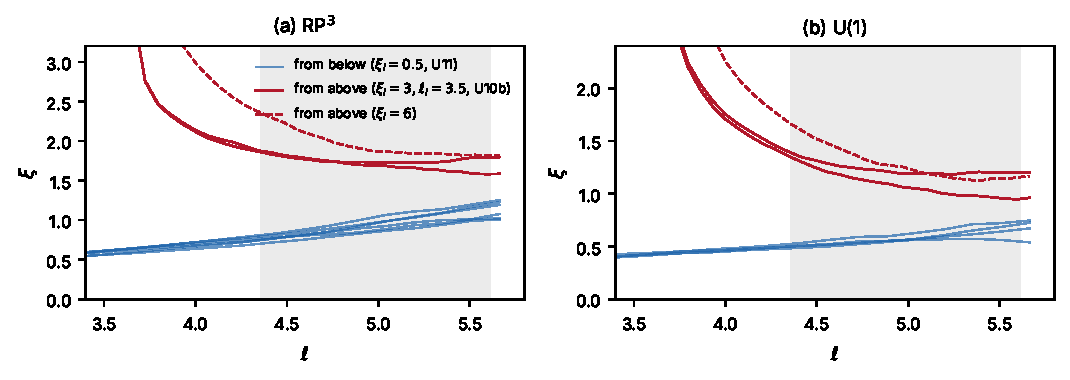
\includegraphics[width=\textwidth]{fig_bracket.pdf}
\caption{The scaling attractor bracketed at $576^3$; each line is one seed. Blue: drained networks starting sparse ($\xi_i=0.5$; six $\RP$ and four U(1) seeds), approaching from below. Red: drained networks started late ($\ell_i=3.5$) and dense (three seeds per model: $\xi_i=3$ solid, two seeds; $6$ dashed, one seed), approaching from above. The shaded band is the analysis window.}
\label{fig:bracket}
\end{figure*}

\subsection{The massive-bath systematic}

Dense starts emit more than sparse ones ($\times1.85$ for $\RP$, $\times1.52$ for U(1)), with a harder spectrum ($q_{\RP}(\ell=5)=0.74\pm0.07$ against $1.03\pm0.12$ with our default convention, though with two dense seeds this difference is convention dependent, \S\ref{sec:results}), and end the window with a $20$--$29\%$ larger ratio of massive to Goldstone energy outside the cores.
Since the density is the same, the excess is unlikely to come from the strings, and two independent tests (below) attribute it to the bath.
The simplest reading is that the initial state leaves a bath of massive radiation that keeps converting into Goldstones inside the window, and that the kinetic estimator counts this conversion as emission.

We tested this in two independent ways.
\emph{Drain:} until $\ell_d=3.8$ the massive part of the velocity (normal to the vacuum manifold) is damped at the physical rate $m_r$, only where the order parameter is close to the vacuum, so cores are untouched; afterwards the evolution is the physical one.
\emph{Exchange:} for U(1) we measure the local transfer from the radial mode to the Goldstone sector, $X=2(\dot r/r)(e_{G,\rm grad}-e_{G,\rm kin})$, which follows from $\partial_te_G=X+\nabla\cdot(r^2\dot\theta\nabla\theta)$ and closes the Goldstone energy budget of a string-free box to $12\%$ (its plane-by-plane analogue for $\RP$ fails that validation and is used only qualitatively).

For the dense U(1) network the drain leaves $43\%$ of the emission, and the undrained exchange attributes $45\%$ to the strings: two methods agree that more than half of the dense-start ``emission'' is bath conversion.
For $\RP$ only an informative comparison is available, drained $512^3$ against undrained $576^3$ dense networks, and it gives the same picture: $43\%$ of the emission remains.
We then repeated the six $\RP$ and four U(1) sparse networks with the same seeds and the bath drained, so that each drained network has an undrained twin (Fig.~\ref{fig:bath}a).
Seed by seed the drain leaves $0.81$ of the $\RP$ emission and $0.72$ of the U(1) one (seed-to-seed scatter $0.05$ and $0.04$): the bath was $19\%$ and $28\%$ of the sparse-start emission.
Because it inflated U(1) more, the undrained $\RG=1.39\pm0.06$ was biased low.
In the drained U(1) networks the measured exchange is below $2.5\%$ of the emission.
Within the window the bath contribution fades: the drained-to-undrained emission ratio of $\RP$ rises by $0.28\pm0.08$ per unit $\ell$ (U(1): $0.04\pm0.03$), while the massive radiation of the network itself, which the drain (switched off at $\ell_d=3.8$) no longer removes, grows.

The drain removes an artefact of the initial state rather than part of the cosmological production: the massive modes decay at tree level well before the late epochs relevant for cosmology, into hard Goldstones that redshift as radiation.
The systematic is, however, intrinsic to the kinetic estimator at accessible $\ell$.
Its size is set mainly by the initial state, not by the number of massive modes: with sparse starts the bath is a smaller share of the emission for $\RP$, with seven massive modes, than for U(1), with one, and with dense starts it is more than half in both.

\begin{figure*}[t]
\centering
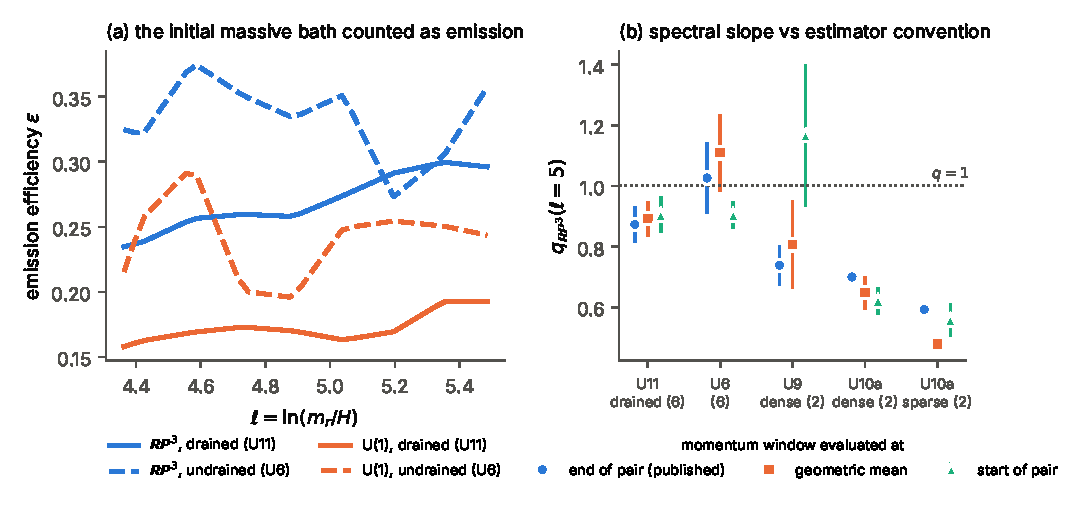
\includegraphics[width=\textwidth]{fig_bath.pdf}
\caption{(a) Emission efficiency (seed means) of the sparse networks with the initial massive bath drained (solid) and of their undrained twins (dashed). (b) Spectral slope $q_{\RP}(\ell=5)$ with bootstrap errors for each data set, with the physical fitting window $[10H,m_r/4]$ converted to lattice momenta using $a$ and $H$ at the end, the geometric middle or the start of each snapshot pair.}
\label{fig:bath}
\end{figure*}

\subsection{Emission and spectrum with the initial bath drained}

With the bath drained (six $\RP$ and four U(1) seeds, $576^3$),
\begin{align}
\RG&=1.56\pm0.09\,({\rm stat})\pm0.08\,({\rm sampling}),\\
\Rxi&=1.61\pm0.06,
\end{align}
that is $\RG=1.56\pm0.12$ with the statistical and snapshot-sampling errors combined, and $\RG=1.54\pm0.09\,({\rm stat})$ when the measured U(1) exchange is subtracted ($1.56$ with the audit's definition of the per-seed exchange fraction).
A preregistered test of the drain at $384^3$ (three seeds) bounds its effect on the ratio: ending it at $\ell_d=3.4$ or $4.1$ instead of $3.8$, or halving or doubling its rate, changes $\RG$ by at most $1.9\pm1.4\%$, which bounds the dependence at the preregistered $5\%$, so we add no drain systematic; the time step stays within its preregistered $2\%$; and in the undrained tests at $\ell\le4.56$ resolution moves $\Rxi$ by $-0.26\%$ and leaves $\RG$ within the sampling systematic, while the volume test shows no dependence larger than its $\approx5\%$ errors. Not quantified are transients beyond the window and the extrapolation to larger $\ell$.
At $512^3$ with two seeds per protocol the drained ratio is $1.63\pm0.02$ for sparse and $1.76\pm0.09$ for dense starts, a protocol gap of $7\%$ against $20\%$ without draining.
Per unit string length the $\RP$ network emits within $13\%$ of U(1) from both sides of the attractor ($\RG/\Rxi=0.97$ from below, $0.87$ from above): the non-abelian network is not radiatively suppressed.
The late dense starts (three seeds per model, $\xi_i=3$, $3$ and $6$ at $\ell_i=3.5$, drained up to $\ell_d=3.8$ as the others) give $\RG=1.30\pm0.14$ and $q_{\RP}(\ell=5)=0.19\pm0.04$ in the same window; they are only $\approx1.5$ e-folds old there, and we read these values as transient rather than as a second measurement of the attractor emission.

For the spectral slope the drained networks give $q_{\RP}(\ell=5)=0.87\pm0.06$, with a weak decrease with $\ell$ ($dq/d\ell=-0.32\pm0.18$), with the window converted to lattice momenta at the end of each snapshot pair.
An independent re-implementation reproduces this number exactly, but finds that the conversion convention matters (Fig.~\ref{fig:bath}b): at the geometric middle or the start of the pair the same data give $0.89\pm0.06$ and $0.90\pm0.06$, and a fit weighted by $F$ gives $0.94\pm0.04$.
The spread is comparable to the statistical error, so the preregistered classification $q<1$ at $2\sigma$ is not robust, and we quote $q$ as compatible with $1$, close to the value reported for U(1) at much larger $\ell$ with adaptive mesh refinement~\cite{Benabou2025} (other U(1) studies find $q$ growing with $\ell$~\cite{GHV2021}).
With two seeds the convention moves $q$ by far more than its bootstrap error (by up to $0.5$ for the dense starts), so earlier two-seed values should be read as $q\approx0.5$--$1.2$.
The sensitivity indicates that the emission spectrum is not a clean power law over the small range $10H<k/a<m_r/4$ available at $\ell\approx5$.

%=====================================================================
\section{Discussion}
%=====================================================================

\paragraph{Comparison with other work.}
Yamada~\cite{Yamada2026} finds scaling ${\rm SU}(2)/\Ztwo$ networks with $\zeta\simeq1.5$ (fixed comoving core) and $2.0$ (physical core, slowly growing), and a density roughly proportional to $N^2-1$.
His $\zeta$ is our $\xi$ (string length from pierced plaquettes with the same factor $2/3$, times $t^2/V$), so absolute densities can be compared: our $\RP$ bracket at $\ell=5.61$, $[1.12,1.73]$, contains his fixed-comoving-core value and lies below his physical-core one, at a different $\ell$ and with different initial conditions.
Our same-code ratio to U(1), $\Rxi\simeq1.6$, is consistent with a denser non-abelian network; the U(1) control density, $\xi\simeq0.6$ at $\ell\simeq5.6$, is on the low side of published values at this $\ell$~\cite{GHV2021,Buschmann2022,Hindmarsh2020scaling,Hindmarsh2021approach}, as expected from our sparse initial conditions, and the late dense starts bracket it.
Our dynamic range ($\ell\le6$) is below the state of the art for U(1) ($\ell\approx8$--$9$)~\cite{Correia2024terasite,Correia2025spectrum}, so our U(1) runs are a control, not a contribution to the scaling dispute.

\paragraph{Implications of the bath systematic for U(1).}
The kinetic estimator is standard in U(1) studies.
A $28\%$ contamination at $\ell\lesssim6$ for sparse starts, and more than half for dense ones, suggests that emission rates and spectra measured at small $\ell$ should be checked against a drained or exchange-corrected estimator, especially where the initial state is far from the vacuum.
In $\RP$ the bath share fades within our window, but in U(1) we see no significant fading ($0.04\pm0.03$ per unit $\ell$ in the drained-to-undrained ratio), so large-$\ell$ simulations should not be assumed free of it.
It is distinct from the contribution of the string fields themselves to the commonly used axion number-density measure, about $30\%$ in large U(1) simulations~\cite{Correia2025spectrum}: the bath is free massive radiation away from the strings.

\paragraph{Limitations.}
(i) The $\RP$ runs reach $\ell=5.66$; nothing here extrapolates to cosmological $\ell\approx70$.
(ii) The drain acts on the network: the drained and undrained $\Rxi$ agree to $0.6\%$, but in the preregistered drain test doubling its rate lowers $\Rxi$ by $5.6\pm1.5\%$, while the emission ratio moves by $1.8\pm1.0\%$ because both models respond alike; the emission per unit string length, $\RG/\Rxi$, therefore moves by about $8\%$, and the $13\%$ agreement with U(1) quoted above carries this drain dependence.
(iii) The exchange $X$ is quantitative only for U(1).
(iv) The slope $q$ depends on the convention for the fitting window and on the type of fit, as shown above.

%=====================================================================
\section{Preregistration, audit and reproducibility}
\label{sec:repro}
%=====================================================================

Each analysis was written as a dated specification (thresholds, windows, estimators, verdict logic) before the corresponding networks were produced, and later changes are dated amendments.
The preregistered verdicts are: attractor gates passed for the U(1) control at $768^3$; genuine growth within the window for sparse and dense starts; an indeterminate verdict for the first drain test at $512^3$ (a residual massive excess); for the drained $576^3$ networks, an emission ratio below the threshold set by the cosmological application ($\RG+\sigma\le1.69$; $\RG+\sigma=1.66$ with the statistical error and $1.68$ with the combined one, a margin of only $0.01$, less than the bound on the drain dependence, so this verdict is marginal) and $q<1$ (the latter not robust, \S\ref{sec:results}); and a bracketed attractor in both models for the late dense starts.
An audit independent of the audited code re-implemented the estimators from the specifications alone, in a separate session without access to the analysis scripts, and reproduced the density, emission and drain numbers of the production networks to $\le4\times10^{-3}$ relative ($\RG$ itself to $2\times10^{-5}$; the later resolution and sampling tests were not audited); it found the $q$ convention dependence reported above and a definitional difference in the per-seed exchange fraction, which leaves $\RG$ unchanged but moves the exchange-corrected value from $1.54$ to $1.56$.
Code, network summaries, specifications, audits and figure scripts are public~\cite{rp3_repo}, and a script there recomputes every number quoted in this paper from the stored results and checks it against the text.
\paragraph{Use of AI tools.} Most of the code, the preregistration documents, the audit and the revisions of this text were produced in an iterative workflow with an AI assistant (Claude Opus 5.5, Anthropic), under the direction of the author, who chose the scientific questions, the model ingredients, the tests and which results to accept.
The audit and the external reviews were carried out in separate sessions of the same assistant or of other assistants, including those of other providers, in a red-teaming approach; the audit above was independent of the audited code but not of the tool.
The output was verified by tests and reproduction checks run in continuous integration, by the re-implementation of the audit, and by the script that recomputes every number in the text; the preregistration was adopted partly to make this workflow checkable.
The author takes full responsibility for the content.

\section{Conclusions}

A global-string network with vacuum manifold $\RP\simeq{\rm SO}(3)$ is $\approx1.6$ times denser than a U(1) network with the same decay constant and core mass, robustly across protocols and from both sides of the attractor, and per unit length it radiates Goldstones within $13\%$ as efficiently, giving $\RG=1.56\pm0.12$ (statistical and snapshot-sampling errors combined) once the initial massive bath is removed.
The bath, counted as emission by the standard kinetic estimator, is a sizeable systematic at accessible $\ell$ ($19$--$28\%$ for sparse starts, more than half for dense ones).
For networks approaching the attractor from below the emission spectrum is close to scale invariant, with a slope at $\ell=5$ that is compatible with $1$ once the estimator convention is accounted for; the late dense starts, still transient, give a much harder spectrum.
With an explicit symmetry-breaking mass the same code also follows the collapse of the string--wall network: in a preliminary measurement (four networks per model at $512^3$, not independently audited) $\RP$ and U(1) leave the same soft Goldstone population per unit string energy, within a ratio of $1.07$, so the denser $\RP$ network yields more quanta only because it has more strings; the collapse and its extrapolation are reported in Ref.~\cite{whalefall_repo}.

\bibliographystyle{apsrev4-2}
\bibliography{refs}

\end{document}
